% Standalone TikZ figure: Unified HDC-LTC Neuron Architecture
% Compile with: pdflatex fig_architecture.tex
\documentclass[tikz,border=5pt]{standalone}
\usepackage{amsmath,amssymb}
\usetikzlibrary{arrows.meta,positioning,calc,decorations.pathreplacing,fit,backgrounds}

\definecolor{hdcblue}{HTML}{0072B2}
\definecolor{ltcorange}{HTML}{E69F00}
\definecolor{gatepurple}{HTML}{CC79A7}
\definecolor{bindgreen}{HTML}{009E73}
\definecolor{bundleyellow}{HTML}{F0E442}
\definecolor{lightgray}{HTML}{F0F0F0}

\newcommand{\bind}{\otimes}
\newcommand{\bundle}{\oplus}

\begin{document}
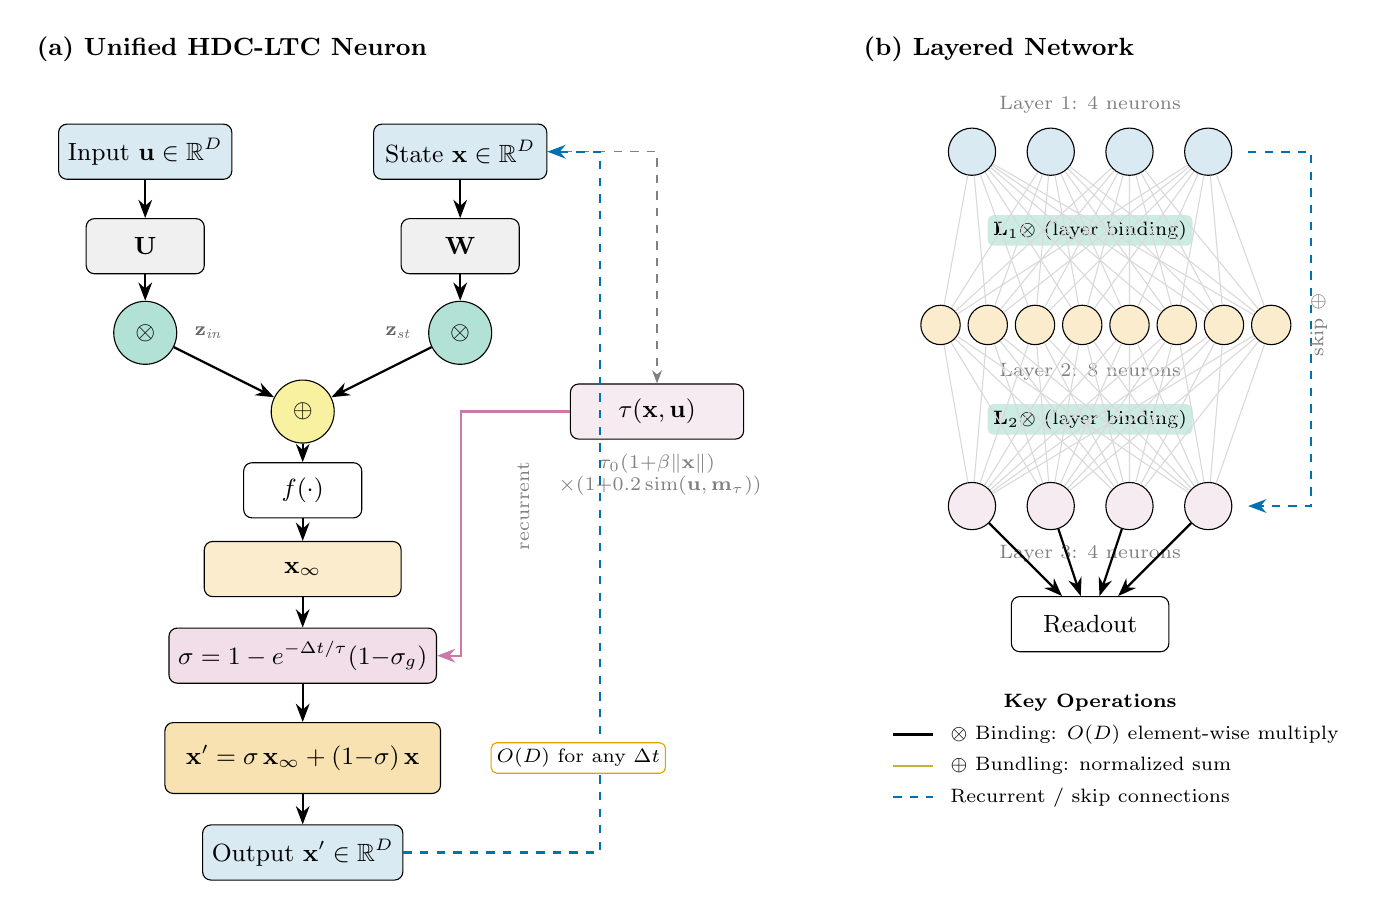
\begin{tikzpicture}[
    >=Stealth,
    node distance=1.2cm and 1.5cm,
    hvbox/.style={draw, rounded corners=3pt, minimum width=2.2cm, minimum height=0.7cm, font=\small},
    opbox/.style={draw, circle, minimum size=0.8cm, font=\small\bfseries, inner sep=0pt},
    label/.style={font=\scriptsize, text=gray},
    hvlabel/.style={font=\scriptsize\itshape, text=black!60},
]

% ============================================================
% LEFT PANEL: Single Neuron Forward Pass
% ============================================================

% Title
\node[font=\small\bfseries, anchor=west] at (-1.5, 5.8) {(a) Unified HDC-LTC Neuron};

% Input and State hypervectors
\node[hvbox, fill=hdcblue!15] (input) at (0, 4.5) {Input $\mathbf{u} \in \mathbb{R}^D$};
\node[hvbox, fill=hdcblue!15] (state) at (4, 4.5) {State $\mathbf{x} \in \mathbb{R}^D$};

% Weight hypervectors
\node[hvbox, fill=lightgray, minimum width=1.5cm] (wu) at (0, 3.3) {$\mathbf{U}$};
\node[hvbox, fill=lightgray, minimum width=1.5cm] (ww) at (4, 3.3) {$\mathbf{W}$};

% Binding operations
\node[opbox, fill=bindgreen!30] (bind1) at (0, 2.2) {$\bind$};
\node[opbox, fill=bindgreen!30] (bind2) at (4, 2.2) {$\bind$};

% Binding labels
\node[hvlabel, right=0.1cm of bind1] {$\mathbf{z}_\text{in}$};
\node[hvlabel, left=0.1cm of bind2] {$\mathbf{z}_\text{st}$};

% Bundle operation
\node[opbox, fill=bundleyellow!50] (bundle) at (2, 1.2) {$\bundle$};

% Activation
\node[hvbox, fill=white, minimum width=1.5cm] (activation) at (2, 0.2) {$f(\cdot)$};

% Equilibrium
\node[hvbox, fill=ltcorange!20, minimum width=2.5cm] (equil) at (2, -0.8) {$\mathbf{x}_\infty$};

% Tau computation (right side)
\node[hvbox, fill=gatepurple!15, minimum width=2.2cm] (tau) at (6.5, 1.2) {$\tau(\mathbf{x}, \mathbf{u})$};
\node[label, text width=2.5cm, align=center] at (6.5, 0.4) {$\tau_0(1{+}\beta\|\mathbf{x}\|)$\\${\times}(1{+}0.2\,\text{sim}(\mathbf{u},\mathbf{m}_\tau))$};

% Gating
\node[hvbox, fill=gatepurple!25, minimum width=2.5cm] (gate) at (2, -1.9) {$\sigma = 1 - e^{-\Delta t/\tau}(1{-}\sigma_g)$};

% Closed-form update
\node[hvbox, fill=ltcorange!30, minimum width=3.5cm, minimum height=0.9cm, font=\small\bfseries] (update) at (2, -3.2) {$\mathbf{x}' = \sigma\,\mathbf{x}_\infty + (1{-}\sigma)\,\mathbf{x}$};

% Output
\node[hvbox, fill=hdcblue!15] (output) at (2, -4.4) {Output $\mathbf{x}' \in \mathbb{R}^D$};

% --- Arrows ---
\draw[->, thick] (input) -- (wu);
\draw[->, thick] (state) -- (ww);
\draw[->, thick] (wu) -- (bind1);
\draw[->, thick] (ww) -- (bind2);
\draw[->, thick] (bind1) -- (bundle);
\draw[->, thick] (bind2) -- (bundle);
\draw[->, thick] (bundle) -- (activation);
\draw[->, thick] (activation) -- (equil);
\draw[->, thick] (equil) -- (gate);
\draw[->, thick] (gate) -- (update);
\draw[->, thick] (update) -- (output);

% Tau arrow to gate
\draw[->, thick, gatepurple] (tau) -| ($(gate.east) + (0.3, 0)$) -- (gate.east);

% State feedback to tau
\draw[->, dashed, gray] (state.east) -| (tau.north);

% Recurrent feedback from output to state
\draw[->, thick, hdcblue, dashed] (output.east) -- ++(2.5, 0) |- (state.east);
\node[label, rotate=90] at (4.8, 0) {recurrent};

% Time annotation
\node[font=\scriptsize, fill=white, draw=ltcorange, rounded corners=2pt, inner sep=2pt] at (5.5, -3.2) {$O(D)$ for any $\Delta t$};

% ============================================================
% RIGHT PANEL: Network Topology
% ============================================================

\node[font=\small\bfseries, anchor=west] at (9, 5.8) {(b) Layered Network};

% Input layer
\node[draw, circle, fill=hdcblue!15, minimum size=0.6cm, font=\tiny] (n11) at (10.5, 4.5) {};
\node[draw, circle, fill=hdcblue!15, minimum size=0.6cm, font=\tiny] (n12) at (11.5, 4.5) {};
\node[draw, circle, fill=hdcblue!15, minimum size=0.6cm, font=\tiny] (n13) at (12.5, 4.5) {};
\node[draw, circle, fill=hdcblue!15, minimum size=0.6cm, font=\tiny] (n14) at (13.5, 4.5) {};
\node[label] at (12, 5.1) {Layer 1: 4 neurons};

% Binding vectors
\node[font=\scriptsize, fill=bindgreen!20, rounded corners=2pt, inner sep=2pt] (lb1) at (12, 3.5) {$\mathbf{L}_1 \bind$ (layer binding)};

% Hidden layer
\foreach \i in {1,...,8} {
    \pgfmathsetmacro{\x}{9.5 + \i * 0.6}
    \node[draw, circle, fill=ltcorange!20, minimum size=0.5cm, font=\tiny] (n2\i) at (\x, 2.3) {};
}
\node[label] at (12, 1.7) {Layer 2: 8 neurons};

% Binding vectors 2
\node[font=\scriptsize, fill=bindgreen!20, rounded corners=2pt, inner sep=2pt] (lb2) at (12, 1.1) {$\mathbf{L}_2 \bind$ (layer binding)};

% Output layer
\node[draw, circle, fill=gatepurple!15, minimum size=0.6cm, font=\tiny] (n31) at (10.5, 0) {};
\node[draw, circle, fill=gatepurple!15, minimum size=0.6cm, font=\tiny] (n32) at (11.5, 0) {};
\node[draw, circle, fill=gatepurple!15, minimum size=0.6cm, font=\tiny] (n33) at (12.5, 0) {};
\node[draw, circle, fill=gatepurple!15, minimum size=0.6cm, font=\tiny] (n34) at (13.5, 0) {};
\node[label] at (12, -0.6) {Layer 3: 4 neurons};

% Connections L1 -> L2 (bundle, so thick)
\foreach \i in {1,...,4} {
    \foreach \j in {1,...,8} {
        \draw[thin, gray!30] (n1\i) -- (n2\j);
    }
}

% Connections L2 -> L3
\foreach \i in {1,...,8} {
    \foreach \j in {1,...,4} {
        \draw[thin, gray!30] (n2\i) -- (n3\j);
    }
}

% Skip connection
\draw[->, thick, hdcblue, dashed] ($(n14.east) + (0.2, 0)$) -- ++(0.8, 0) |- ($(n34.east) + (0.2, 0)$);
\node[label, rotate=90] at (14.9, 2.3) {skip $\bundle$};

% Readout
\node[hvbox, fill=white, minimum width=2cm] (readout) at (12, -1.5) {Readout};
\draw[->, thick] (n31) -- (readout);
\draw[->, thick] (n32) -- (readout);
\draw[->, thick] (n33) -- (readout);
\draw[->, thick] (n34) -- (readout);

% Legend
\begin{scope}[shift={(9, -2.8)}]
    \node[font=\scriptsize\bfseries] at (3, 0.3) {Key Operations};
    \draw[thick] (0.5, -0.1) -- (1.0, -0.1); \node[font=\scriptsize, anchor=west] at (1.1, -0.1) {$\bind$ Binding: $O(D)$ element-wise multiply};
    \draw[thick, bundleyellow!80!black] (0.5, -0.5) -- (1.0, -0.5); \node[font=\scriptsize, anchor=west] at (1.1, -0.5) {$\bundle$ Bundling: normalized sum};
    \draw[thick, dashed, hdcblue] (0.5, -0.9) -- (1.0, -0.9); \node[font=\scriptsize, anchor=west] at (1.1, -0.9) {Recurrent / skip connections};
\end{scope}

\end{tikzpicture}
\end{document}
